\chapter{Introducción}

En este capítulo se presenta una introducción a los sistemas UWB, sus
características y aplicaciones. Asimismo, se analizan posibles implementaciones
prácticas de dichos sistemas basadas en arquitecturas clásicas de sistemas de
radiofrecuencia de banda angosta, y las limitaciones que las mismas poseen
cuando son aplicadas a sistemas UWB. A continuación se analizan arquitecturas
alternativas concebidas específicamente para sistemas UWB y sus beneficios con
respecto a los sistemas clásicos de banda angosta, para luego analizar de qué
modo pueden simplificarse las arquitecturas y al mismo tiempo aumentar su
desempeño si se utilizan circuitos específicos con la mirada puesta en un
sistema UWB. Uno de los circuitos de mayor importancia en estas arquitecturas es
el generador de pulsos ultracortos, Se analizaran los resultados reportados en
la literatura con respecto a estos circuitos, dentro de los cuales resalta la
topología basada en diodo SRD serie con linea de transmisión en paralelo por su
bajo costo de implementación. Luego, se analizarán aplicaciones del generador de
pulsos propuesto en los caminos de recepción y transmisión de una plataforma UWB
de referencia \cite{Altieri2021}. Por último, se llegará a un conjunto de
especificaciones para el generador de pulsos a desarrollar.

\section{Introducción a UWB}

La tecnología UWB (del inglés \textit{Ultra Wide Banda}, ultra ancho de banda)
es una tecnología de radio caracterizada por la transmisión y recepción de
señales de ancho de banda muy elevado. Como contrapartida, en el dominio del
tiempo dichas señales son de muy corta duración. Esto es contraposición a los
sistemas de RF usuales, que suelen ser de banda angosta o sintonizados. Las
señales temporales ultracortas o el ancho de banda grande supone un desafío para
el diseño de los sistemas.

Para dar una definición precisa de un sistema UWB consideramos la definida por
la Comisión Federal de Comunicaciones de los Estados Unidos (FCC por sus siglas
en inglés) que define un sistema UWB como uno en el que el ancho de banda
utilizado es mayor a \qty{500}{\mega\hertz} o \qty{20}{\percent} de la
frecuencia portadora \cite{FCC_UWB}. Para la definición de ancho de banda, la
comisión utiliza la definición de ancho de banda a \qty{10}{\dB}, en lugar de
los \qty{3}{\dB} usuales en otros campos. De esta manera el ancho de banda queda
definido como la franja de frecuencia en la que la potencia cae \qty{10}{\dB}
con respecto al punto de máxima potencia.

En las tecnologías de radio de banda angosta, que componen la mayoría de las
asignadas por la FCC, se asigna un ancho de banda pequeño relativo a la
frecuencia de la portadora. Debido al gran ancho de banda de los sistemas UWB,
es inevitable que el rango de frecuencias se superponga con alguno asignado a
otra tecnología. Para evitar interferencia excesiva, sobre todo con sistemas
críticos como el GPS, la FCC asigna una máscara espectral sobre la potencia
máxima permitida para los sistemas UWB. En la figura \ref{fig:fcc_uwb_psd_mask}
puede observarse la misma.  La máscara se establece sobre la PIRE, Potencia
Isotrópica Radiada Equivalente (o EIRP del inglés \textit{Equivalent Isotropic
Radiated Power}). Esta cantidad es la potencia que debería emitir un radiador
isotrópico para realizar la misma intensidad de radicación en la dirección de
máxima potencia de la antena. Es una medida de direccionalidad de la antena que
permite comparar entre radiadores con distintos patrones de radiación.

\begin{figure}[t]
    \centering
    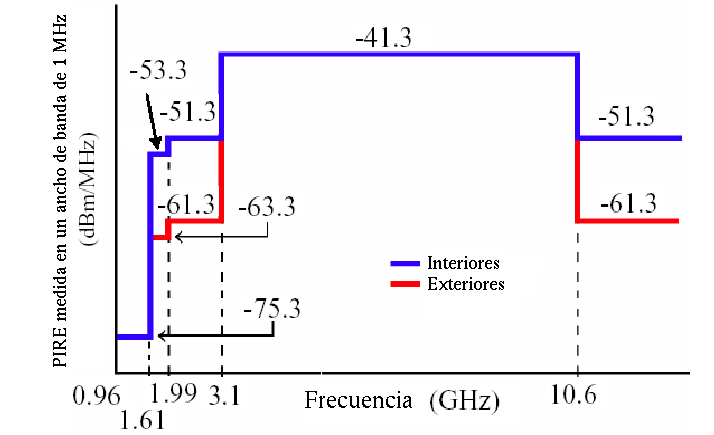
\includegraphics[width=0.7\textwidth]{images/fcc_uwb_psd_mask.png}
    \caption{Máscara de PSD para señales UWB establecida por la FCC. Tomada de \cite{Heydari2005}.}
    \label{fig:fcc_uwb_psd_mask}
\end{figure}

La tecnología UWB encuentra aplicaciones en diversas areas

\begin{itemize}
  \item \textbf{Radar:} El gran ancho de banda de las señales UWB se presta
        para aplicaciones de radar que requieran de gran resolución espacial. Su
        capacidad de penetración profunda permite aplicaciones de radar en las
        que se pueden resolver objetos bloqueados por paredes. Su gran
        penetración también permite aplicaciones en GPR (del inglés
        \textit{Ground Penetrating Radar}, radar de penetración de suelo), en
        las que la señal de radar se utiliza para identificar materiales
        enterrados en el suelo o dentro de muros. Algunos ejemplos
        pueden consultarse en \cite{morales2018}, \cite{savelyev2010},
        \cite{senapati2021}.
  \item \textbf{Comunicaciones:} Otra ventaja del gran ancho de banda de estos
        sistemas es la capacidad de transmisión de datos que puede obtenerse.  En
        sistemas de transmisión de datos de corto alcance, pueden explotarse las
        propiedades de las señales UWB para obtener altas tasas de transmisión.
        Algunos ejemplos son \cite{jaesang2004}, \cite{zhiquan2005},
        \cite{Heydari2005}
  \item \textbf{Imágenes médicas:} Existen aplicaciones en las que radares de
        impulsos Doppler UWB son utilizados para medición de signos vitales
        críticos como pulso cardíaco y respiración. Este tipo de radares frente
        a otros de onda continua presentan ventajas como menor consumo y mayor
        resolución. Algunos ejemplos son \cite{jalivand2011}, \cite{oloumi2020},
        \cite{jalivand2011_2}.
  \item \textbf{Caracterización de materiales:} ciertos materiales pueden ser
      caracterizados mediante su iluminación con una señal UWB y un análisis
        sobre las reflexiones de la señal. El gran ancho de banda de esta
        respuesta permite realizar caracterizaciones del material que con
        señales de banda angosta no serían posibles. Algunos ejemplos de estas
        aplicaciones pueden consultarse en \cite{altieri2017},
        \cite{Salman2008}, \cite{Bouza2023}, \cite{Muqaibel2003},
        \cite{salman2010performance}, \cite{Altieri2021}
\end{itemize}

Como se ha mostrado, los sistemas UWB tienen numerosas aplicaciones en la
práctica. En este contexto, debemos diferenciar aquellas aplicaciones de consumo
masivo, donde se espera producir un gran número de unidades de un sistema, y
aquellas aplicaciones más específicas o experimentales, que no se desarrollan a
gran escala. Para las primeras, de escala industrial, puede ser razonable el
desarrollo de un circuito integrado específico que permita amortizar los costos
de desarrollo con el volumen. Para la segundas, específicamente para las
aplicaciones experimentales, es más conveniente contar con un sistema de menor
costo no integrado, que permita realizar pruebas y sea adaptable a diversas
aplicaciones. Este es el contexto en el que se desarrollará la presente tesis.

\section{Sistemas UWB basados en generadores de pulsos ultracortos}

A continuación, se describirá una propuesta de sistema UWB basado en un
generador de pulsos ultracortos. Se partirá de un sistema reportado en la
literatura \cite{Altieri2021} basado en generación de pulsos en banda base y
conversión a banda pasante mediante un multiplicador de frecuencias. Se
describirá la plataforma reportada, y se detallará cómo un generador de pulsos
ultracortos permite una fuerte simplificación del sistema implementado, y cómo
las diversas métricas de desempeño del sistema están fuertemente asociadas a los
parámetros del pulso.

En el trabajo de referencia \cite{Altieri2021} se desarrolló una plataforma para
la estimación del contenido de humedad en poliamidas en base a señales UWB, es
decir, una aplicación de caracterización de materiales. En esta aplicación, un
objeto a caracterizar es irradiado por una cadena de pulsos periódica y se
reciben múltiples copias de la respuesta del blanco. Luego, a partir de estas
copias es posible realizar caracterizaciones sobre el material mediante técnicas
de detección y estimación.  Para que esta estimación sea exitosa, es fundamental
que el contenido espectral de los pulsos sea lo más amplio posible.

En cuanto a la arquitectura de la plataforma reportada, la misma contiene
entonces dos caminos, el de transmisión y el de recepción. El diagrama en
bloques de ambos puede observarse en la figura
\ref{fig:uwb_system_block_diagram}.  La arquitectura de dicha plataforma es
análoga a la de un sistema tradicional de transmisión y recepción de banda
angosta. La señal a transmitir es generada primero en banda base, y luego
modulada a banda pasante mediante una portadora.  En el sistema receptor la
señal es convertida a banda base nuevamente y muestreada en tiempo real con un
conversor analógico-digital que cumpla con el criterio de Nyquist. No obstante
existen algunas diferencias con la arquitectura de un sistema de banda angosta.
Por un lado, la conversión a banda base se realiza en un solo salto, a
diferencia de los sistemas tradicionales de comunicaciones que en general
utilizan varias frecuencias intermedias. En un sistema de banda angosta es
conveniente realizar varios saltos, dado que en cada etapa se incrementa el ancho
de banda relativo de la señal (que es muy pequeño), permitiendo diseñar etapas
de filtrado menos selectivas. En un sistema UWB esto es contraproducente porque,
a diferencia de un sistema de banda angosta, el ancho de banda relativo es muy
elevado, y una conversión a frecuencia intermedia lo incrementaría, haciendo más
complejo el sistema. Por otra parte, los sistemas de banda angosta no trasladan
a la señal de banda pasante a frecuencia cero para su muestreo como el sistema
UWB, sino que trabajan con una frecuencia intermedia no nula y las señales son
muestreadas en dicha banda, realizando el lazo de sincronización por medio de
procesamiento digital. Esto es impracticable en el caso del sistema UWB de modo
la señal se demodula directamente a frecuencia cero, con los inconvenientes
prácticos que ello puede generar.

A continuación se detallará como un generador de pulsos ultracortos permite
simplificar la implementación de las cadenas de transmisión y recepción del
sistema UWB de referencia. En ambos caminos, se detallará cómo se reducen los
costos tanto económicos de los componentes cómo de desarrollo de los sistemas.

\begin{figure}[t]
    \centering
    \begin{subfigure}[b]{0.45\textwidth}
        \centering
        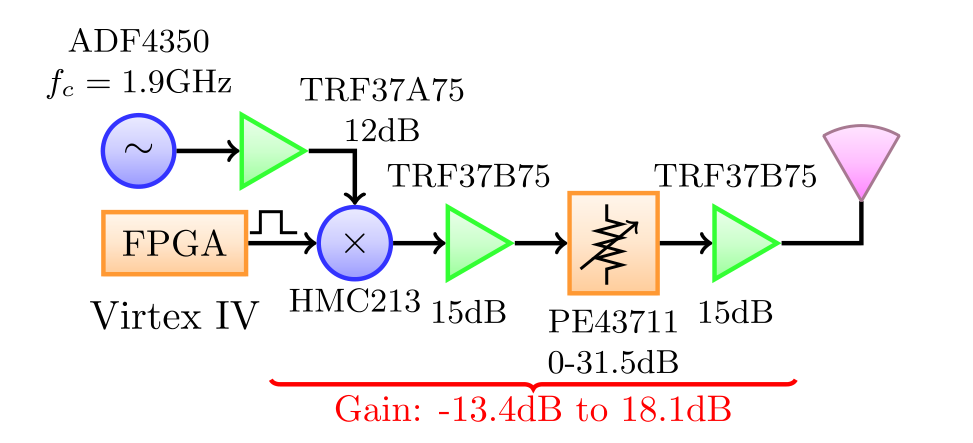
\includegraphics[width=\textwidth]{images/uwb_system_tx_path.png}
        \caption{Camino de transmisión en plataforma UWB. Tomado de
        \cite{Altieri2021}.}
        \label{fig:uwb_system_tx_path}
    \end{subfigure}
    \hfill
    \begin{subfigure}[b]{0.45\textwidth}
        \centering
        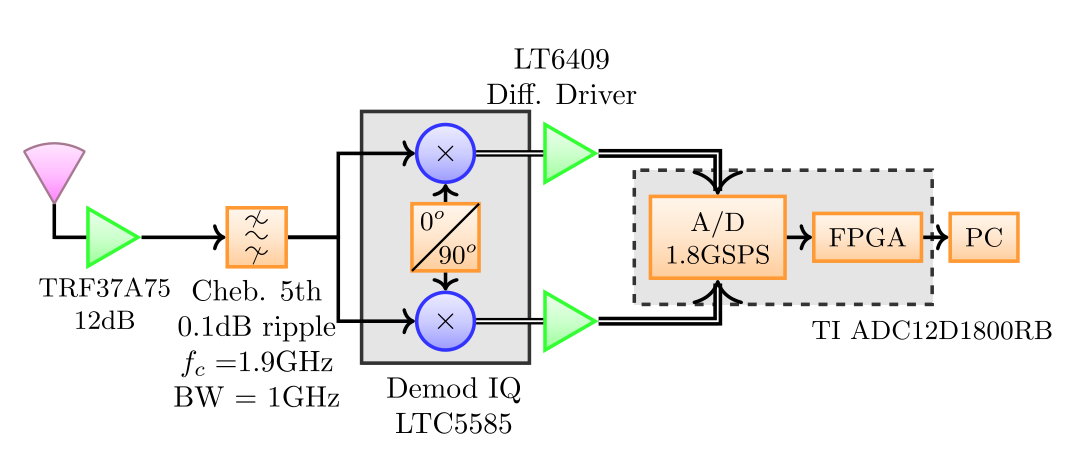
\includegraphics[width=\textwidth]{images/uwb_system_rx_path.png}
        \caption{Camino de recepción en plataforma UWB. Tomado de
        \cite{Altieri2021}.}
        \label{fig:uwb_system_rx_path}
    \end{subfigure}
        \caption{Cadenas de transmisión y recepción en sistema UWB reportado en
        \cite{Altieri2021}.}
    \label{fig:uwb_system_block_diagram}
\end{figure}

\subsection{Aplicaciones en transmisión}

El diagrama en bloques del camino de transmisión puede observarse en la figura
\ref{fig:uwb_system_tx_path}. La función de esta cadena es generar un pulso en
banda pasante a ser transmitido por la antena, que irradiará sobre el objeto a
caracterizar. En este caso, se toma una frecuencia central de transmisión de
\qty{1.9}{\giga\hertz} y un ancho de banda de \qty{1}{\giga\hertz}. Para la
transmisión de este pulso en banda pasante, se parte de un pulso generado por
una FPGA. Este pulso tiene un ancho mínimo dado por el reloj mínimo del sistema,
que en este caso se encontraba en \qty{1.5}{\nano\second}, con un ancho de banda
de \qty{10}{\dB} de \qty{1.28}{\giga\hertz}. Este pulso se encuentra en banda
base, para pasarlo a banda pasante se utiliza un multiplicador de frecuencia
pasivo. Para la multiplicación es necesaria una señal de referencia de
\qty{1.9}{\giga\hertz}, y dado que el multiplicador es pasivo, este requiere que
la potencia de la referencia sea de \qty{13}{\dBm}.  Para lograr esto se
requiere de un oscilador activo y un amplificador para lograr la potencia
necesaria. Dado que el multiplicador es pasivo y tiene una pérdida especificada
en \qty{10}{\dB}, es necesario un bloque de ganancia para compensar. En este
caso, se utilizaron dos bloques de ganancia intercalados por un atenuador
configurable, de manera de darle a todo el sistema una ganancia configurable de
entre \qty{-13.4}{\dB} y \qty{18.1}{\dB}.

A continuación se explicará cómo esta cadena puede ser fuertemente simplificada
con un generador de pulsos ultracortos. En la figura
\ref{fig:proposed_uwb_tx_path} se observa la cadena de señal propuesta. Para
generar el pulso en banda pasante, en lugar de utilizar una arquitectura basada
en una generación de pulso en banda base y luego una modulación a banda pasante,
se utilizará una basada en un generador de pulsos y un filtro pasabanda. El
pulso en banda pasante de la arquitectura original se encontraba en una
frecuencia central de \qty{1.9}{\giga\hertz} con un ancho de banda de
\qty{1}{\giga\hertz}. Para generar este pulso, se propone una arquitectura en la
que se dispone de un filtro pasabanda con las características del pulso deseado,
es decir, una frecuencia central de \qty{1,9}{\giga\hertz} y
\qty{1}{\giga\hertz} de ancho de banda, y se lo excita con un pulso ultra corto.
Este pulso aproxima a un impulso ideal, siendo que excitar un sistema LTI con un
impulso ideal resulta en una señal con un espectro igual a la función
transferencia del sistema, en este caso la salida tendrá el espectro del filtro
pasabanda. Por ser el ancho del pulso finito y distinto de 0, la salida no será
exactamente igual a la transferencia del filtro, pero con un pulso lo
suficientemente corto es suficiente. En terminos de frecuencia, es suficiente
con que el ancho de banda a \qty{10}{\dB} sea mayor a la máxima frecuencia útil,
en este caso $ \qty{1,9}{\giga\hertz}+ \qty{1}{\giga\hertz}/2 =
\qty{2,4}{\giga\hertz}$. Para mantener la funcionalidad de ganancia variable,
entre el pulser y el filtro pasabanda se incluyen un amplificador y un atenuador
variable.

De esta manera, se implementa una cadena que requería de 6 componentes por una
que solo requiere de 2. En el caso de la arquitectura propuesta, la potencia de
salida puede ser ajustada con la amplitud del generador de pulsos, ya que la
misma define la amplitud del pulso en banda pasante. Regulando la amplitud de
este generador se regula la potencia. En cuanto a la forma espectral del pulso
de salida, es controlable por el filtro pasabanda, lo que presenta una gran
versatilidad además de baja complejidad.  Cabe resaltar la importancia del
generador en esta cadena, que debe generar pulsos ultracortos (tales que su
ancho de banda sea mayor al de los pulsos en banda pasante) y amplitud
regulable. En caso de ser necesario, pueden agregarse un amplificador y
atenuador variable como se indica en la figura \ref{fig:proposed_uwb_tx_path}
para darle más versatilidad al ajuste de amplitud.

Además de la menor cantidad de componentes en la arquitectura propuesta, estos
son más simples. En la arquitectura original se necesita, además de los
amplificadores y el atenuador variable, un oscilador y un multiplicador, ambos
componentes con significativas complejidades de implementación y limitaciones
asociadas.

\begin{itemize}
    \item El oscilador requiere un diseño de una placa especial, y el diseño de
        la misma es de complejidad ya que el camino del  oscilador es crítico en
        el desempeño del sistema. También requiere de un control digital, ya sea
        en un microcontrolador, con el costo asociado al desarrollo del
        programa. Además, la salida es de baja potencia, lo que requiere un
        amplificador adicional.
    \item En cuanto al multiplicador, dado el gran ancho de banda de las señales
        de trabajo, es necesario utilizar uno pasivo. Estos son dispositivos no
        lineales, en general de menor desempeño que los activos adaptados a
        señales de banda angosta.  Estos multiplicadores requieren portadoras de
        potencia (\qty{10}{\dBm}-\qty{15}{\dBm}) considerable que el oscilador
        por defecto no alcanza, por lo que es necesario un amplificador. Ademas
        tienen restricciones del ancho de banda en banda base, y restricciones
        del ancho de banda en banda pasante; además no deben superponerse las
        bandas. Por ejemplo, en el HMC213 utilizado en la plataforma de
        referencia \cite{Altieri2021}, la banda de entrada es hasta
        \qty{1.5}{\giga\hertz}, y la banda pasante es de
        \qty{1.5}{\giga\hertz}-\qty{4.5}{\giga\hertz}. Entonces si se quiere
        pasar una señal de \qty{1}{\giga\hertz} en banda base, al modularla
        queda con \qty{2}{\giga\hertz} en banda pasante, la portadora mínima
        debe ser \qty{2.5}{\giga\hertz} para evitar que se superponga la banda
        de entrada con la banda pasante).
\end{itemize}

En la arquitectura propuesta, no es necesario el multiplicador y, por lo tanto,
tampoco el oscilador. Removiendo estos componentes se elimina gran parte del
costo monetario y de ingeniería de la plataforma, ya que como fuese descripto
anteriormente, estos dos componentes involucran múltiples restricciones y
complejidades en la implementación. En la cadena de transmisión propuesta, la
mayor complejidad está en la implementación del pulser. Una vez diseñado este
componente, la etapa de transmisión solamente necesita el diseño del filtro
pasabanda, que puede ser realizado directamente con una línea de transmisión en
la placa, y opcionalmente la inclusión de un amplificador comercial.

\begin{figure}[t]
    \centering
    \begin{subfigure}[b]{0.45\textwidth}
        \centering
        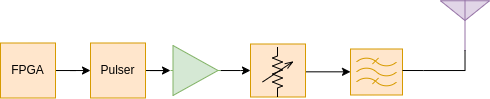
\includegraphics[width=\textwidth]{images/proposed_uwb_tx_path.drawio.png}
        \caption{Propuesta de camino de transmisión en plataforma UWB basado en
        generador de pulsos ultra cortos.}
        \label{fig:proposed_uwb_tx_path}
    \end{subfigure}
    \hfill
    \begin{subfigure}[b]{0.45\textwidth}
        \centering
        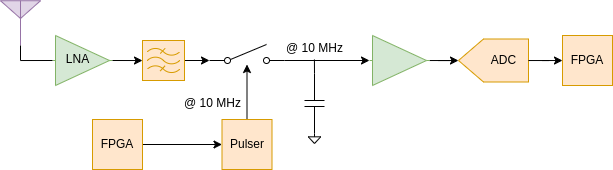
\includegraphics[width=\textwidth]{images/proposed_uwb_rx_path.drawio.png}
        \caption{Propuesta de camino de recepción en plataforma UWB basado en
        generador de pulsos ultra cortos.}
        \label{fig:proposed_uwb_rx_path}
    \end{subfigure}
    \caption{Propuestas de cadenas de transmisión y recepción en sistema UWB
    basado en generador de pulsos ultracortos.}
    \label{fig:uwb_system_block_diagram}
\end{figure}

\subsection{Aplicaciones en recepción}

En cuanto al receptor, en la figura \ref{fig:uwb_system_rx_path} se observa la
cadena de señal implementada en la plataforma de referencia. La misma está
compuesta por un amplificador de bajo ruido como primer etapa, seguido de un
filtro pasabanda antialiasing. Luego del filtrado se realiza una conversión a
banda base con un demodulador I/Q, seguido de una amplificación. Finalmente se
realiza una conversión A/D con un conversor de tiempo real con tasa de muestreo
de \qty[per-mode=symbol]{1.8}{\giga\siemens\per\second}. Este conversor de
tiempo real vuelve muy costoso al sistema, ya que un conversor de tan alta tasa
de muestreo tiene un ancho de banda analógico muy grande, lo que vuelve el costo
tanto monetario como de desarrollo de ingeniería muy alto.  Como referencia, el
circuito integrado de dicho conversor AD, el ADC12D1800 de Texas Instruments
\footnote{\url{https://www.ti.com/product/ADC12D1800}},
tiene un costo unitario superior a 1800 dolares, a lo que deben sumarse costos
de desarrollo adicionales.

Explotando la periodicidad de la señal recibida, es posible simplificar esta
cadena reemplazándola por una basada en un generador de pulsos ultracortos,
realizando en lugar de muestreo en tiempo real un muestreo en tiempo
equivalente, técnica posibilitada por la periodicidad de la señal de entrada. En
este esquema, se muestrea a una tasa mucho menor a la de Nyquist, muestreando la
señal en distintos puntos de su período. Luego, estos puntos pueden ser
alineados correctamente para reconstruir la señal original. En la figura
\ref{fig:Illustration_of_equivalent_time_sampling} puede observarse el esquema.
Se observa como se toman muestras a una tasa mucho menor a la de Nqyuist, con el
cuidado de en cada muestra tomar un punto distinto dentro de la forma de onda a
muestrear. De esta manera, el conversor en tiempo real de gran tasa de muestreo
puede ser reemplazado por un conversor de baja tasa y bajo costo, reduciendo de
manera importante el costo del sistema.

Con el muestreo en tiempo equivalente es posible muestrear una señal a una tasa
mucho menor a la de Nyquist. Sin embargo, un conversor A/D de la baja tasa de
muestreo deseada tiene un ancho de banda analógico bajo, por lo que no sería
posible muestrear directamente el pulso en banda pasante. Para hacer de interfaz
entre esta señal y el conversor de baja tasa, es posible implementar un circuito
de \textit{Sample \& Hold} que muestrea la señal, proveyendo al conversor una
señal discretizada de bajo ancho de banda. En la figura
\ref{fig:sampling_circuit} se observa un circuito de muestreo basado en pulsos
ultra cortos reportado en \cite{han2004}. El mismo se basa en diodos para
muestrear la señal, que son accionados por pulsos ultracortos. La duración
temporal de estos pulsos define el ancho de banda máximo de entrada. La amplitud
determina el rango dinámico.

Con este esquema basado en muestreo en tiempo equivalente e implementado con un
circuito de muestreo basado en diodos de muestreo accionados por pulsos ultra
cortos, es posible reemplazar al costoso conversos de tiempo real de la figura
\ref{fig:uwb_system_rx_path} por el circuito propuesto. De esta manera, se llega
a una cadena de recepción como la de la figura \ref{fig:proposed_uwb_rx_path}.
En este sistema, se mantienen como primeras etapas el amplificador de bajo ruido
y el filtro pasabanda. Estos componentes son de bajo costo y de baja complejidad
de implementación. Luego, en lugar del demodulador I/Q, los amplificadores
diferenciales y el conversor de Nyquist, se encuentra el circuito de muestreo
excitado por el pulser. Los pulsos de control del circuito de muestreo
trabajarían a una frecuencia de repetición PRF (del inglés \textit{Pulse
Repetition Frequency}) de \qty{10}{\mega\hertz}. A la salida del muestreador se
realizaría una forma de onda compuesta por las muestras del pulso en banda
pasante. Esta señal es amplificada por un amplificador operacional de bajo ancho
de banda y muestreada por un ADC de baja tasa, siendo la necesaria de
\qty[per-mode=symbol]{10}{\mega\siemens\per\second}, más de 2 ordenes de
magnitud por debajo de la tasa del conversor de la figura
\ref{fig:uwb_system_rx_path}.

\begin{figure}[t]
    \centering
    \begin{subfigure}[b]{0.45\textwidth}
        \centering
        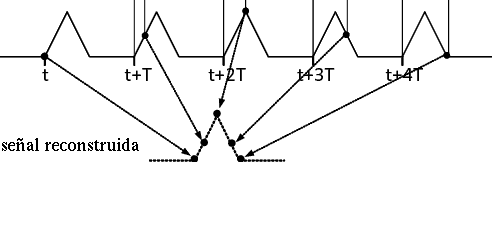
\includegraphics[width=\textwidth]{images/Illustration-of-equivalent-time-sampling.png}
        \caption{Ilustración de la técnica de muestreo en tiempo equivalente.}
        \label{fig:Illustration_of_equivalent_time_sampling}
    \end{subfigure}
    \hfill
    \begin{subfigure}[b]{0.45\textwidth}
        \centering
        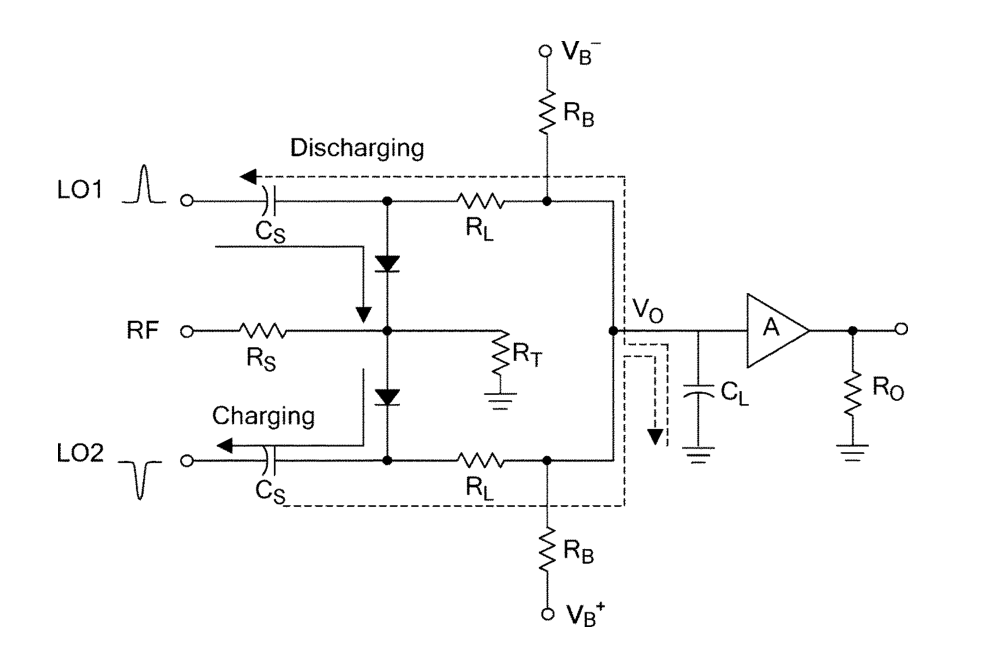
\includegraphics[width=\textwidth]{images/sampling_circuit.png}
        \caption{Circuito de muestreo basado en pulsos ultra cortos. Tomado de
        \cite{han2004}.}
        \label{fig:sampling_circuit}
    \end{subfigure}
    \caption{Esquema de muestreo en tiempo equivalente y circuito de muestreo
    reportado en \cite{han2004}.}
    \label{fig:equivalent_time_sampling_figures}
\end{figure}

\subsection{Requerimientos del generador de pulsos}

En base a las posibles aplicaciones en los caminos de transmisión y recepción de
pulsos de una plataforma UWB, se determina el conjunto de
especificaciones de la tabla \ref{tab:pulser_requirements} para el generador de
pulsos. Este conjunto fue determinado con el objetivo de lograr un generador lo
más económico y simple posible, teniendo como restricción su aplicabilidad a la
plataforma de referencia \cite{Altieri2021}. Esto impone los requerimientos de
amplitud y duración temporal de pulso y de interfaz con el sistema. El
requerimiento de simplicidad no impacta directamente en la tabla de requisitos
sino en la arquitectura que se seleccionará para el generador.

El requisito de $V_{in}$ en la tabla \ref{tab:pulser_requirements} se refiere a
la entrada de control del pulser. Esta se corresponde con una salida digital de
la FPGA, que trabaja en \qty{3.3}{\volt}.  Esta salida digital es de baja
capacidad de carga, por lo que la entrada tiene que tener un bajo consumo de
corriente. Para $V_{dd}$ se admite un valor superior a los \qty{3.3}{\volt} de
la FPGA, y se apunta a una alimentación regulable entre \qty{5}{\volt} y
\qty{5}{\volt}.

En cuanto a las características del pulso, se espera un FWHM (del inglés
\textit{Full Width at Half Maximum}) de alrededor de \qty{120}{\pico\second}.
Esta ancho temporal permite trabajar en los anchos de bandas de la plataforma de
referencia \cite{Altieri2021}, tanto como para el camino de transmisión como el
de recepción. En cuanto a la amplitud, una de entre \qty{500}{\milli\volt} y
\qty{1.5}{\volt} es suficiente. Cuanto mayor sea la amplitud, menor la
complejidad de implementación de las aplicaciones, ya que si esta es suficiente
se pueden ahorrar amplificadores. De todas maneras, si la amplitud no es lo
suficientemente grande, un amplificador no representa un gran costo para el
sistema. La PRF de los pulsos se espera que sea de \qty{10}{\mega\hertz}. Esto
permite en el camino de recepción propuesto muestrear la salida del muestreador
con un ADC de baja tasa.

\begin{table}
\centering
\begin{tabular}{c|c}
\hline
    Variable & Requerimiento \\
\hline
    $V_{in}$                &   CMOS @ $V_{DD}=\qty{3.3}{\volt}$ ($V_{OH}$
    \qty{2.4}{\volt})     \\
    PRF                &        \qty{10}{\mega\hertz} \\
    $V_{dd}$                &   \qty{5}{\volt} - \qty{8}{\volt} \\
    $A$                &        \qty{500}{\milli\volt}-\qty{1.5}{\volt} \\
    FWHM                &       \qty{120}{\pico\second} \\
\hline
\end{tabular}
\caption{Requerimientos del generador de pulsos.}
\label{tab:pulser_requirements}
\end{table}

\section{Generadores de pulsos ultracortos}

Como fuese explicado anteriormente, un componente fundamental de los sistemas
UWB es el generador de pulsos ultracortos. Un generador de pulsos de buenas
características de FWHM y amplitud permite simplificar fuertemente sistemas UWB
basados en implementaciones tradicionales. Para esto, es fundamental en este tipo
de generadores lograr anchos de pulso menores a \qty{1}{\nano\second} y tener
amplitudes variables. En esta sección se explorarán las distintas arquitecturas
reportadas en la literatura para generadores de pulsos, y se seleccionará una en
base a los requisitos expuestos anteriormente.

Existen diversas topologías para la implementación de estos circuitos. En la
literatura se encuentran resultados reportados con implementaciones tanto
integradas como discretas. En los generadores implementados en circuitos
integrados, son usuales las arquitecturas basadas en la suma de una señal de
entrada con distintos niveles de retardo, generado pulsos con forma de gaussiana
derivada \cite{Nguyen2012} \cite{Salehi2010} \cite{An2018}. Como se mencionó
anteriormente, el objetivo es contar con un sistema UWB modular para
aplicaciones experimentales por lo que serán de interés para nosotros analizar
las arquitecturas con componentes discretos, que no requieran el diseño de un
circuito integrado.

En la familia de generadores implementados con componentes discretos,
prácticamente la totalidad de los resultados reportados en la literatura se
encuentran implementados en base a diodos SRD \cite{rulikowski2004}
\cite{protiva2009} \cite{kamal2014} \cite{oloumi2020} \cite{han2005}. Estos
generadores presentan buen desempeño en cuanto a amplitud de pulso y duración
temporal, además de extremadamente baja complejidad de implementación. Dado que
este tipo de generador cumple con los requerimientos de complejidad y dado los
resultados reportados demuestra ser capaz de lograr los requisitos detallados en
la tabla \ref{tab:pulser_requirements}, este será el tipo de generador a
implementar en este trabajo. A continuación se detallarán las principales
características de los mismos, las distintas topologías existentes y sus
ventajas y desventajas.

\subsection{Generadores basados en diodo SRD}

Como fuese explicado anteriormente, prácticamente la totalidad de los
generadores de pulsos ultracortos implementados con componentes discretos
reportados en la literatura están basados en diodos SRD. Este tipo de
dispositivos pertenecen a la familia de diodos de almacenamiento de carga. Se
diferencian por su característica de recuperación reversa, presentando esta un
largo tiempo de almacenamiento seguido de un tiempo de transición muy corto, lo
que permite su aplicación en generación de pulsos ultracortos.
Constructivamente, estos diodos son diodos PIN, es decir, diodos compuestos por
un material semiconductor intrínseco entre dos semiconductores P y N. A
diferencia de los diodos PIN utilizados en circuitos de radiofrecuencia y
microondas como llaves activas, los diodos SRD tienen una capa I muy fina,
propiedad que los dota de su anteriormente mencionada característica de
recuperación reversa.

Los generadores basados en diodo SRD se caracterizan por su bajo costo,
versatilidad en cuanto a amplitud y ancho de pulso y baja complejidad de
implementación. Este tipo de generadores contienen al diodo SRD, en algunos
casos ningún otro componente semiconductor o activo \cite{Zhang2006}
\cite{rulikowski2004} \cite{han2005} y en la mayoría de los casos otro
componente semiconductor pasivo con el objetivo de rectificar o adaptar la forma
de onda \cite{protiva2009} \cite{kamal2014} \cite{han2002}. Aunque el generador
de pulsos no necesita componentes activos, suelen ser necesarios en etapas
\textit{driver} previas a la generación de pulso o en etapas de amplificación
posteriores a la generación. De todas formas, el generador es extremadamente
simple, basándose solamente el diodo SRD, una red de polarización y
opcionalmente otro semiconductor pasivo para mejorar la forma del pulso. Las
etapas anteriores y posteriores al generador dependerán de la integración con el
resto del sistema.  Es por estos motivos que son ampliamente utilizados en la
generación de pulsos para sistemas UWB.

Existen distintas arquitecturas de generación de pulsos basados en este diodo.
En todas el finamiento se basa en la característica de recuperación reversa,
estando presente las variaciones en el tipo de componentes utilizados, el tipo
de señal de entrada y su acople y la forma de utilización del diodo. En la mayor
parte de los generadores reportados en la literatura, se puede diferenciar entre
SRD serie o paralelo con la señal, y la utilización de inductores o líneas de
transmisión en paralelo, o \textit{stub}, para la generación del pulso.

Clasificaremos entonces a los generadores en dos grupos según su topología:
serie y paralelo. A continuación serán explicadas las ventajas y desventajas de
cada grupo.

\begin{figure}
    \centering
    \begin{subfigure}[b]{0.45\textwidth}
        \centering
        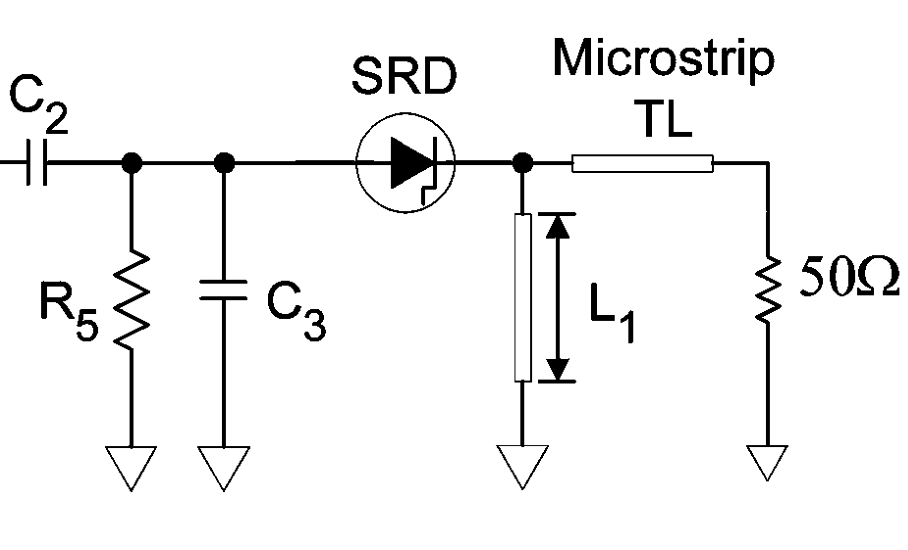
\includegraphics[width=\textwidth]{images/srd_series_generator.png}
        \caption{Generador SRD serie. Tomado de \cite{han2005}.}
        \label{fig:srd_series_generator}
    \end{subfigure}
    \hfill
    \begin{subfigure}[b]{0.45\textwidth}
        \centering
        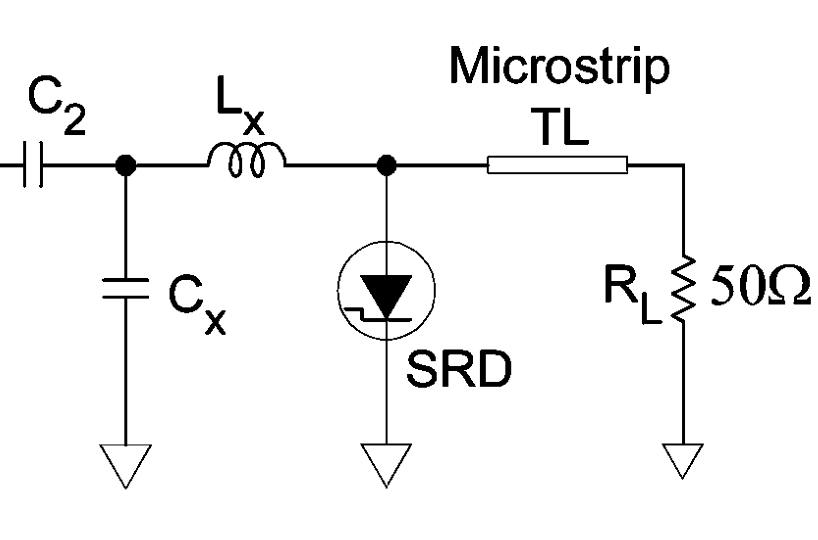
\includegraphics[width=\textwidth]{images/srd_shunt_generator.png}
        \caption{Generador SRD paralelo. Tomado de \cite{han2005}.}
        \label{fig:srd_shunt_generator}
    \end{subfigure}
    \caption{Generadores de pulsos basados en SRD con topología serie y
    paralelo.}
    \label{fig:srd_pulse_generator_topologies}
\end{figure}

\subsubsection{Serie}

En los generadores que denominaremos serie, el diodo SRD se encuentra en serie
con la señal. En la figura \ref{fig:srd_series_generator} se observa un ejemplo.
En este caso, el diodo SRD genera un flanco muy rápido en base a uno
(posiblemente) lento, Con este flanco rápido, se utiliza un stub cortocircuitado
a tierra para reflejarlo y así lograr un pulso ultra corto. La duración temporal
de este pulso estará dado por el retardo de propagación en la línea de
transmisión, mientras que la amplitud estará determinada por el retardo en la
línea, la amplitud de la señal de entrada y la velocidad de crecimiento del
flanco generado por el SRD. La señal de entrada puede estar acoplada de manera
directa al diodo, o acoplada en alterna. El primer tipo de acople tiene asociado
una mayor disipación de potencia, mientras que la segunda presenta menor
disipación pero más complejidad de implementación, ya que la correcta
polarización del diodo y su transición al estado de alta impedancia se vuelven
más desafiantes.

Estos generadores se caracterizan por su simplicidad de implementación. El hecho
de utilizar una línea de transmisión para la generación del pulso simplifica el
diseño, ya que no requiere la adquisición de componentes adicionales, siendo que
la selección de los mismos es desafiante en el contexto de UWB dónde se debe
trabajar en grandes anchos de banda. La utilización de la línea de transmisión
permite controlar el ancho de pulso con los parámetros de la línea, que son
función de los materiales utilizados y de la geometría de la misma, lo que
elimina la dependencia del ancho de pulso en componentes externos.

Se encuentran reportados trabajos sobre generadores serie que permiten
configurar la duración de pulso \cite{Zhang2006}. Esto se logra intercalando en
la línea de transmisión múltiples diodos PIN puestos a tierra, conectados por
tensiones de control. De esta manera, el largo efectivo de la línea puede
reducirse polarizando los diodos PIN. Esta estrategia no se tomará en este
trabajo ya que es preferible un generador simple a uno reconfigurable, pero es
un aspecto interesante a tener en cuenta en futuras iteraciones.

\subsubsection{Paralelo}

En los generadores paralelo, el diodo SRD se encuentra en paralelo con la
salida. El SRD presenta una baja impedancia mientras se encuentra polarizado en
directa. Una vez aplicada una corriente inversa para conmutar al dispositivo a
su estado de alta impedancia, el mismo permanece en el estado de baja impedancia
durante un tiempo denominado tiempo de almacenamiento. Extinguido este período,
el diodo transiciona al estado de alta impedancia en un tiempo dado por su
tiempo de transición, que para diodos SRD es del orden de picosegundos. Teniendo
al diodo en paralelo con la salida, es posible generar un pulso ultra corto en
base a esta transición. Para lograr esto, se coloca en serie un inductor que
genera una resonancia con la capacidad a tierra del diodo SRD \cite{Hall1966}.
Esta frecuencia de resonancia se relaciona con el ancho de pulso y permite su
control.

En la literatura se reportan mejores amplitudes de pulso para los generadores
paralelo que para los serie \cite{han2005}. Sin embargo, esta mayor amplitud
trae como contrapartida la mayor complejidad de implementación asociada con la
presencia de un inductor en el camino de la señal. La selección de este
componente debe ser cuidadosa, ya que por los anchos de banda de trabajo los
componentes deben tener un gran ancho de banda. En el caso del generador serie,
se utiliza una línea de transmisión sobre la que se tiene mayor control con
respecto a sus parámetros. Es por esta razón que para este trabajo se adoptará
una arquitectura basada en diodo SRD serie, siendo preponderante la simplicidad
de implementación sobre la amplitud de pulso.


\section{Organización del trabajo}

En el presente trabajo se diseñará un generador de pulsos ultracortos con
las aplicaciones desarrolladas anteriormente en caminos de transmisión y
recepción de sistemas UWB. El objetivo de este generador es simplificar estas
cadenas de señal. Para lograr este objetivo, se determinó un conjunto de
especificaciones resumidas en la tabla \ref{tab:pulser_requirements}. Para
lograr un generador simple y de bajo costo, se optó por una arquitectura basada
en diodo SRD utilizando la topología serie.

Habiendo determinado el alcance y los objetivos del trabajo, se detallará cómo
se organizará el trabajo. En el capitulo 2 se explicará en detalle el
funcionamiento del diodo SRD, los fenómenos físicos que determinan su
funcionamiento, sus parámetros principales y se estudiarán los modelos de
simulación disponibles. En el capitulo 3 se estudiará la aplicación de diodos
SRD en circuitos aceleradores de flanco, y como estos en combinación con una
línea de transmisión cortocircuitada conforman un circuito generador de pulsos.
Se analizará para este circuito la dependencia de los parametros del pulso con
los componentes del circuito. Una vez diseñado el circuito generador, se
describirá el desarrollo de una etapa driver. Finalmente, se reporta  la
implementación física de estos circuitos en PCB. En el capitulo 4 se presentarán
las mediciones realizadas sobre el circuito y se reportarán resultados de
simulaciones sobre aplicaciones del generador en las cadenas de transmisión y
recepción propuestas para el sistema UWB. Finalmente, en el capitulo 5 se
presentarán las conclusiones obtenidas y posibles trabajos a futuro.

La metodología de trabajo para el diseño de circuitos se basará en la obtención
de expresiones simbólicas para las cantidades de interés, acompañadas de
simulaciones validando las expresiones obtenidas. A lo largo de este trabajo,
para las simulaciones será utilizado el software \textit{Advanced Design System}
o ADS por sus siglas en inglés, de la compañía Keysight
\footnote{\url{https://www.keysight.com/us/en/products/software/pathwave-design-software/pathwave-advanced-design-system.html}}.
Se utiliza este programa por sus buenas prestaciones en lo que respecta a
circuitos de radiofrecuencia y microondas. Eventualmente se utilizará también el
software LTspice
\footnote{\url{https://www.analog.com/en/design-center/design-tools-and-calculators/ltspice-simulator.html}}
en ciertas ocasiones en las que ADS no sea suficiente.
